\documentclass{beamer}
\usepackage[francais]{babel}
\usepackage[T1]{fontenc}
\usepackage[utf8]{inputenc}  
\usepackage{verbatim} 
\usepackage{indentfirst}          %pour \verbatiminput{fich}
\usetheme{JuanLesPins}    % titre en haut
\useoutertheme{default}       
\setlength{\parindent}{0.5cm}

\graphicspath{{Figures/}}
\setbeamertemplate{caption}[numbered] % pour numéroter tables et figures !
%si \verb   : \begin{frame}[fragile]
%si verbatim  : \begin{frame}[containsverbatim]


\title{La robotique}
\author{Jérémy SIMIONE, Thomas BESSON , Leif HENRIKSEN}
\institute{Université de Montpellier}
\date{2019}

\begin{document}
% Premier transparent de titre
\begin{frame}
  \titlepage
\end{frame}

% 2eme transparent TDM générale
\AtBeginSection[]
{
    \begin{frame}
        \frametitle{Sommaire}
        \tableofcontents[currentsection,hideothersubsections]
    \end{frame}
}

\section{Microcontrôleur, nano-ordinateur : le cerveau du robot}
\subsection{ Microcontrôleur}
\begin{frame}
\frametitle{Définition}
\begin{block}{Définition}
Un microcontrôleur est un circuit intégré qui rassemble les éléments essentiels d'un ordinateur.
 Les microcontrôleurs se caractérisent par un plus haut degré d'intégration, une plus faible consommation électrique,
 une vitesse de fonctionnement plus faible  et un coût réduit par rapport aux microprocesseurs  utilisés dans les ordinateurs personnels. 
\end{block}
\end{frame}
\begin{frame}
\frametitle{Composition d'un microcontrôleur}
  Les composants d'un microcontrôleur sont :
  \begin{itemize}
      \item Un processeur ou un microprocesseur 
      \item De la mémoire vive (RAM) 
      \item De la mémoire morte (ROM) 	
      \item Des périphériques, capables d'effectuer des tâches spécifiques. On peut mentionner  :
		\begin{itemize}
   			\item Les convertisseurs analogiques-numériques (CAN) 
 			  \item Les convertisseurs numériques-analogiques (CNA) 
 			  \item Les contrôleurs de bus de communication
		\end{itemize} 
  \end{itemize}
\end{frame}
\begin{frame}
\frametitle{Programmation d'un microcontrôleur}
\begin{itemize}
\item À l'origine, les microcontrôleurs se programmaient en assembleur (problèmes de maintenance).
\item Désormais, on utilise de plus en plus des langages de haut niveau, notamment le langage C.
\item Avec l’augmentation de la puissance et de la quantité de mémoire de stockage (FLASH) , les programmes  peuvent désormais être écrits en C++. 
\item Il existe même des frameworks et plateformes en C++ destinés à l’embarqué, comme Qtopia, mais l'utilisation de ceux-ci restera limitée aux microcontrôleurs les plus puissants. 
\end{itemize}
\end{frame}
\begin{frame}
\frametitle{Programmation d'un microcontrôleur : suite}
\begin{itemize}
\item  Pour programmer le microcontrôleur, il est alors possible d'utiliser différents langages de programmations tels que:
\begin{itemize}
  \item BASIC
  \item C
  \item C++
  \item JAVA
  \end{itemize}
\end{itemize}
\begin{itemize}
  \item Le programme réalisé dans le langage de haut niveau est compilé dans le langage assembleur conçu par le constructeur du microcontrôleur. Puis ce programme ainsi compilé sera injecté du PC dans la mémoire programmable du microcontrôleur.
\end{itemize}
\end{frame}
\subsection{Nano-ordinateurs, ordinateurs mono-carte}
\begin{frame}
\frametitle{Défintion}
 \begin{block}{Définition}
 Un ordinateur à carte unique ou ordinateur mono-carte est un ordinateur complet construit sur un circuit imprimé,
 avec un ou plusieurs microprocesseur(s), de la mémoire, des lignes d'entrée/sortie et d'autres éléments pour en faire un ordinateur fonctionnel. 
 \end{block}
\end{frame}
\begin{frame}
\frametitle{Nano ordinateur ou microcontrôleur?}
\begin{itemize}
\item Si un nano-ordinateur a l’apparence d’un microcontrôleur, il est utile de rappeler que ce dernier peut être qualifié de nano-ordinateur dans la mesure où il:
\begin{itemize}
    \item Permet de faire fonctionner un système d’exploitation de haut niveau, comme par exemple Windows, Android ou Linux .
    \item Intègre ou il permet de connecter à minima des périphériques d’affichage (écran, télévision) et de saisie (clavier physique ou virtuel, souris ou écran tactile).
    \item Comporte un moyen de stockage dédié (disque dur, carte SD, clé usb) et possède un port ethernet.
    \item Fonctionne de manière autonome, sans nécessité de le raccorder à un autre ordinateur.
   \item Jusqu'a 40 fois plus rapide qu'un microcontroleur
\end{itemize}
\end{itemize}
\end{frame} 
\begin{frame}
\frametitle{Programmation d'un nano-ordinateur}
\begin{itemize}
    \item Au niveau de la programmation le nano-ordinateur pourra etre programmé dans n'importe quel langage de haut niveau et l'IDE pourra etre choisi car il comporte son propre systeme d'exploitation a contrario du microcontrôleur.
    \item L'injection du code dans le nano-ordinateur se fera par un outil de transfert du PC au nano-ordinateur.
\end{itemize}
\end{frame}	
\begin{frame}
\frametitle{Exemple de microcontrôleur et nano-ordinateur}
\begin{figure}[!h]
\centering
\includegraphics[width=6cm]{BANANA_PI_01.jpg}
\caption{Un nano ordinateur, le banana PI}
\end{figure}
\end{frame}
\begin{frame}
\frametitle{Exemple de microcontrôleur et nano-ordinateur}
\begin{figure}[!h]
\centering
\includegraphics[width=6cm]{expose.jpg}
\caption{Un microcontrôleur}
\end{figure}
\end{frame}
\subsection{Les choix : conclusion}
\begin{frame}
\frametitle{Les choix : conclusion}
\begin{itemize}
    \item La différence entre un microcontrôleur et un nano-ordinateur réside donc dans le fait qu'un nano-ordinateur est en fait un vrai PC avec  des periphériques intégrés, contrairement au microcontroleur qui sera plus approprié dans le cas de taches industrielles repetitives.
  \item Un microcontrôleur sera par exemple adapté a un robot qui trie des skittles (robot industiel) , alors qu'un robot avec assistance vocale (ex: androide) aura besoin d'une connexion internet pour fonctionner ce qui est donc plus adapté a un nano-ordinateur.
\item Pour conclure le cerveau du robot peut être créée soit avec un nano-ordinateur soit avec un microcontrôleur le choix sera effectué en fonction des besoins du robot.
\end{itemize}
\end{frame}

\section{Exemples de Robot}
\subsection{Les Humanoïdes}
\begin{frame}
\frametitle{Robots Humanoïdes}
\begin{itemize}
    \item C'est l'un des types de robot le plus connue aujourd'hui.
    \begin{figure}
        \centering
        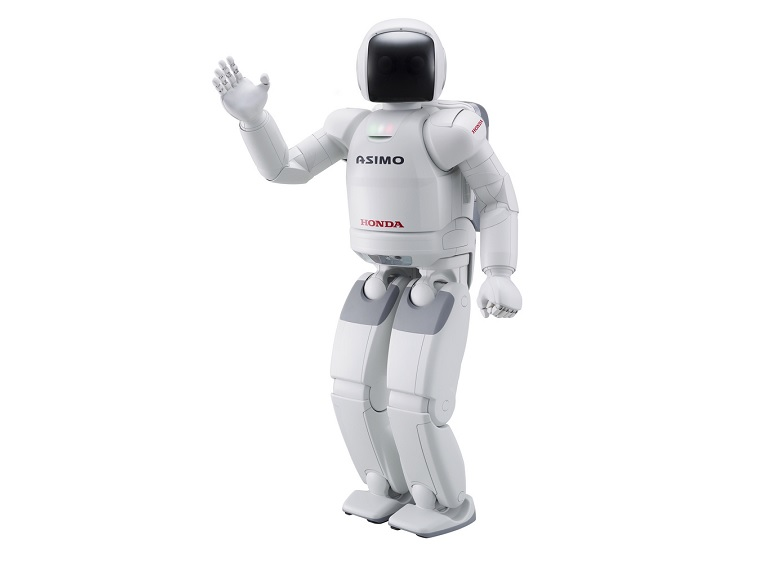
\includegraphics[width=100]{img/asimo.png}
        \caption{Robot Asimo de chez Honda}
        \label{fig:my_label}
    \end{figure}
    \item Un robot Humanoïde est un robot qui a la morphologie d'un humain. 
    \item Certains robot Humanoïdes ne représentent que une partie du corps humain. 
\end{itemize}
\end{frame}
\begin{frame}
\begin{itemize}
    \item Malgrès tout certains robot ont l'apparence d'un humain ou le comportement d'un humain :
    \begin{figure}
        \centering
        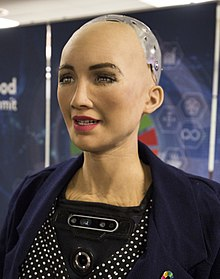
\includegraphics[width=100]{img/sophia.png}
        \caption{Sophia}
        \label{fig:my_label}
    \end{figure}
    
\end{itemize}
    
\end{frame}
\subsection{Robots informatique}
\begin{frame}{Robots Informatiques}
\begin{itemize}
    \item On le connais surtout sous le nom de bot informatique. 
    \item Un bot est un programme informatique qui peut être utilisé à différentes fins.
    \item C'est un agent logiciel qui interagit automatiquement avec des serveurs informatiques.
    \begin{figure}
        \centering
        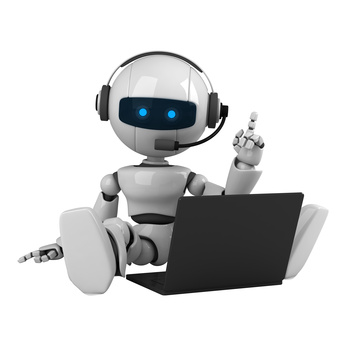
\includegraphics[width=100]{img/bot.png}
        \label{fig:my_label}
    \end{figure}
    
\end{itemize}
\end{frame}

\begin{frame}{Robots Informatiques}
\begin{itemize}
    \item Exemple de bot, recevoir un message de confirmation pour la réception d'un colis.
    \item On utilise les bots dans différents domaine comme le web et le jeu vidéo.
    \item Il n'y a pas de meilleur langage pour créer un bot, tout dépend de votre utilisation du bot. 
\end{itemize}
\end{frame}
\subsection{Les Robots Industriels}
\begin{frame}{Robots Industriels}

\begin{itemize}
    \item Le but d'un robot industriel est de réaliser des tâches et de manipuler des objets automatiquement. 
    \begin{figure}
        \centering
        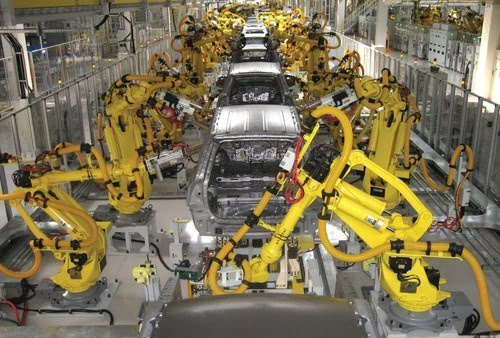
\includegraphics[width=200]{img/auto.png}
        \caption{Constructeur Automobile}
        \label{fig:my_label}
    \end{figure}
    
\end{itemize}
\end{frame}

\begin{frame}
\item Ils sont plus rapide et plus précis que des humains et aussi ne se fatiguent jamais. 
\item A la base les robots industriels étaient utilisés dans le nucléaire. \begin{figure}
        \centering
        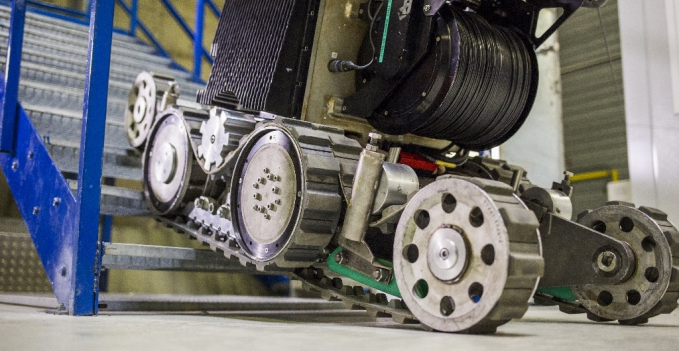
\includegraphics[width=200]{img/nucl.png}
        \caption{Robot Nucléaire français MERIT}
        \label{fig:my_label}
    \end{figure}
    
\end{frame}

\begin{frame}{Conclusion}
    \begin{figure}
        \centering
        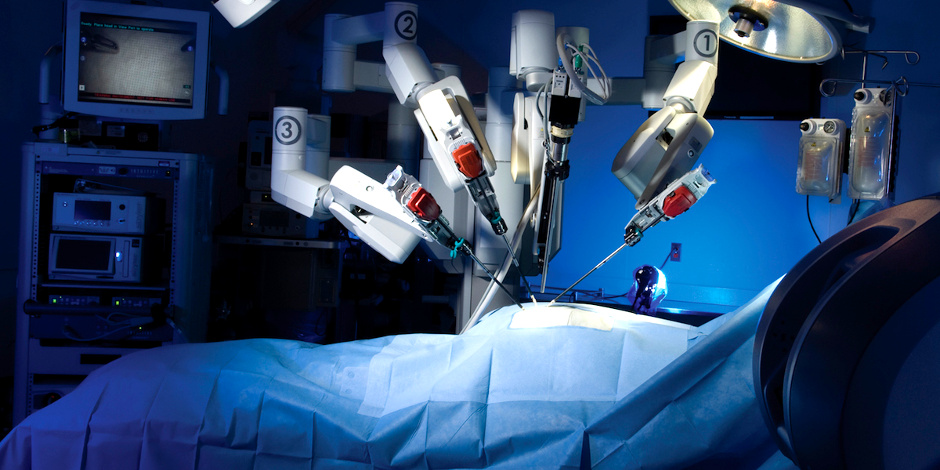
\includegraphics[width=125]{img/chirg.png}
        \caption{Robot chirugicale}
        \label{fig:my_label}
    \end{figure}
    \begin{figure}
        \centering
        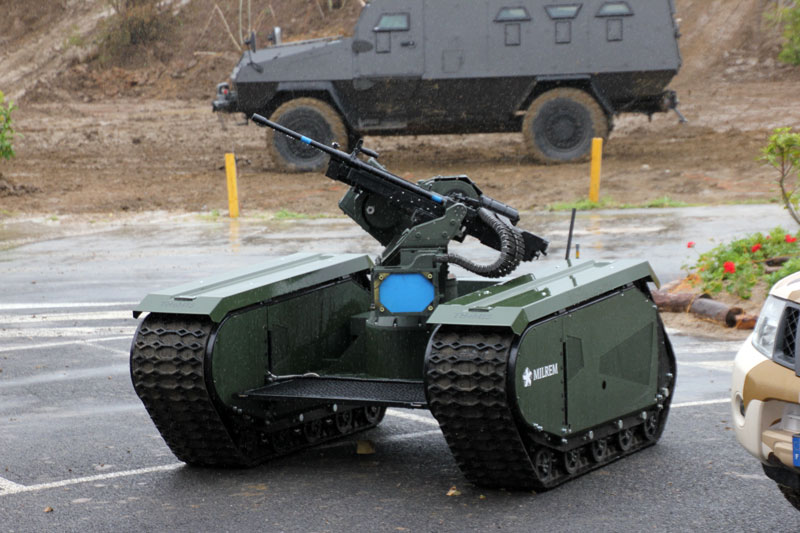
\includegraphics[width=125]{img/militaire.png}
        \caption{Robot Militaire} 
        \label{fig:my_label}
    \end{figure}
\end{frame}
\end{document} 